\subsection{Balanced Gray code and Z3 SMT solver}
\label{Gray_Z3}

\renewcommand{\CURPATH}{gray_code/SMT}

Suppose, you are making a rotary encoder.
This is a device that can signal its angle in some form, like:

\begin{figure}[H]
\centering
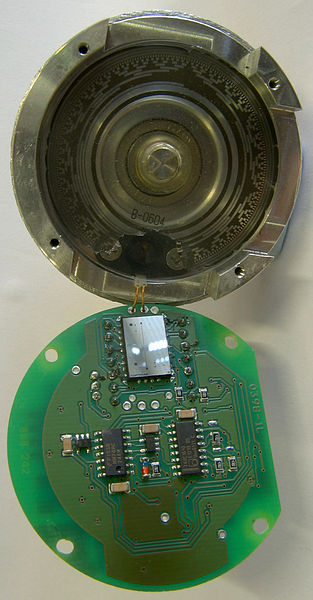
\includegraphics[scale=1]{\CURPATH/313px-Gray_code_rotary_encoder_13-track_opened.jpg}
\caption{Rotary encoder}
\end{figure}

( The image has been taken from Wikipedia: \url{https://en.wikipedia.org/wiki/Gray_code} )

% TODO FIX URL
Click on \href{.../blog/gray/Gray_code_rotary_encoder_13-track_opened.jpg}{bigger image}.

This is a rotary (shaft) encoder: \url{https://en.wikipedia.org/wiki/Rotary_encoder}.

\begin{figure}[H]
\centering
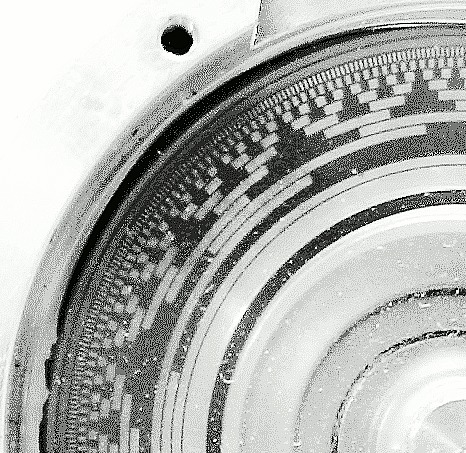
\includegraphics[scale=0.8]{\CURPATH/Rotary_Encoder_track_detail_scaled_crop.jpg}
\caption{Cropped and photoshopped version}
\end{figure}

( Source: \url{http://homepages.dordt.edu/~ddeboer//S10/304/c_at_d/304S10_RC_TRK.HTM} )

% TODO FIX URL
Click on
\href{.../Rotary_Encoder_track_detail.jpg}{bigger one}.

There are pins and tracks on rotating wheel.
How would you do this?
Easiest way is to use binary code.
But it has a problem: when a wheel is rotating, in a moment of transition from one state to another, several bits may be changed, hence, undesirable state may be present for a short period of time.
This is bad.
To deal with it, Gray code was invented: only 1 bit is changed during rotation.
Like:

\begin{lstlisting}
Decimal Binary  Gray
0 	0000 	0000
1 	0001 	0001
2 	0010 	0011
3 	0011 	0010
4 	0100 	0110
5 	0101 	0111
6 	0110 	0101
7 	0111 	0100
8 	1000 	1100
9 	1001 	1101
10 	1010 	1111
11 	1011 	1110
12 	1100 	1010
13 	1101 	1011
14 	1110 	1001
15 	1111 	1000
\end{lstlisting}

Now the second problem. Look at the picture again. It has a lot of bit changes on the outer circles.
And this is electromechanical device.
Surely, you may want to make tracks as long as possible, to reduce wearing of both tracks and pins.
This is a first problem.
The second: wearing should be even across all tracks (this is balanced Gray code).

How we can find a table for all states using Z3:

\lstinputlisting{\CURPATH/gray.py}

% TODO FIX URL
( The source code: \url{...gray.py} )

For 4 bits, 4 changes is enough:

\lstinputlisting{\CURPATH/4.txt}

% TODO FIX URL
8 changes for 5 bits: \url{.../5.txt}.
12 for 6 bits (or maybe even less): 
\url{.../6.txt}.

\subsubsection{Duke Nukem 3D from 1990s}

\begin{figure}[H]
\centering
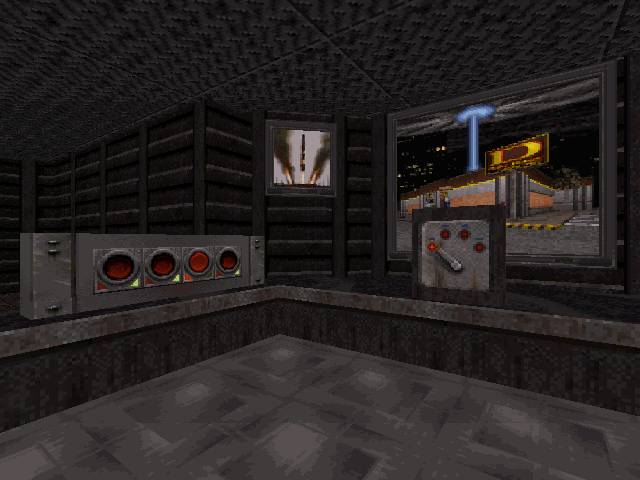
\includegraphics[scale=3]{\CURPATH/duke.png}
\caption{Duke Nukem 3D}
\end{figure}

Another application of Gray code:

\begin{lstlisting}
with.inspiring@flair.and.erudition (Mike Naylor) wrote:

>In Duke Nukem, you often come upon panels that have four buttons in a row,
>all in their "off" position. Each time you "push" a button, it toggles from
>one state to the other. The object is to find the unique combination that
>unlocks something in the game.

>My question is: What is the most efficient order in which to push the
>buttons so that every combination is tested with no wasted effort?

A Gray Code. :-)

(Oh, you wanted to know what one would be?  How about:
0000
0001
0011
0010
0110
0111
0101
0100
1100
1101
1111
1110
1010
1000
1001
1011

Or, if you prefer, with buttons A,B,C,D: D,C,D,B,D,C,D,A,D,C,D,B,C,D,C
It isn't the "canonical" Gray code (or if it is, it is by Divine
Providence), but it works.

Douglas Limmer -- lim...@math.orst.edu
"No wonder these mathematical wizards were nuts - went off the beam -
he'd be pure squirrel-food if he had half that stuff in _his_ skull!"
E. E. "Doc" Smith, _Second Stage Lensmen_
\end{lstlisting}

( \url{https://groups.google.com/forum/#!topic/rec.puzzles/Dh2H-pGJcbI} )

Obviously, using our solution, you can minimize all movements in this ancient videogame, for 4 switches, that would be 4*4=16 switches.
With our solution (balanced Gray code), wearing would be even across all 4 switches.

